% ICDV 2026 Paper
% GNNocRoute: Topology-Aware Periodic Routing Optimization for NoC
% 6 pages, IEEE double-column
% Deadline: 30 May 2026

\documentclass[conference]{IEEEtran}
\usepackage{cite}
\usepackage{amsmath,amssymb,amsfonts}
\usepackage{graphicx}
\usepackage{textcomp}
\usepackage{xcolor}
\usepackage{booktabs}
\usepackage{array}
\usepackage{multirow}
\usepackage{hyperref}
\usepackage{caption}
\usepackage{footnote}

\hypersetup{colorlinks=true,linkcolor=blue,citecolor=blue,urlcolor=blue}
\graphicspath{{./figures/}}

\begin{document}

\title{GNNocRoute: Topology-Aware Periodic Routing Optimization for Network-on-Chip using Graph Neural Networks}

\author{
    \IEEEauthorblockN{Le Tien Hieu\textsuperscript{1}, \textit{IEEE Member}}
    \IEEEauthorblockA{\textsuperscript{1}Institute of Information Technology (VNU-ITI),\\
    Vietnam National University, Hanoi, Vietnam\\
    Email: letienhieu@mcs.edu.vn}
}

\maketitle

\begin{abstract}
Network-on-Chip (NoC) is the communication backbone for modern multi-core System-on-Chips. Conventional deterministic routing algorithms such as XY dimension-order routing suffer from significant congestion imbalance---our graph-theoretic analysis across seven topologies shows that an $8\times8$ mesh with XY routing achieves congestion imbalance of 0.475, with central nodes exhibiting $2-3\times$ higher betweenness centrality than edge nodes.

We present a feasibility study on topology-aware periodic routing optimization for NoC using Graph Neural Networks (GNN). We report four experimental findings. First, GNN embeddings strongly correlate with betweenness centrality ($|r|$ up to 0.978). Second, cross-topology experiments show that relative node importance rankings transfer across mesh sizes (Pearson $r \approx 0.96$). Third, measured inference latency ($\approx 10^6$ cycles on CPU) confirms that periodic optimization is necessary. Fourth, cycle-accurate simulations (BookSim2, 480 runs, 5 seeds, 95\% CI) show that adaptive routing reduces hotspot latency by up to 23\% compared to XY routing.
\end{abstract}

\begin{IEEEkeywords}
Network-on-Chip, Graph Neural Networks, Adaptive Routing, Congestion Analysis, Periodic Optimization
\end{IEEEkeywords}

% ══════════════════════════════════════════════════════════════
\section{Introduction}
\label{sec:intro}

Network-on-Chip (NoC) has become the standard communication infrastructure for modern multi-core SoCs and AI accelerators such as Google TPU and NVIDIA Grace Hopper~\cite{mirhoseini2021}. The routing algorithm determines packet paths and directly affects system performance in terms of latency, throughput, and energy consumption.

As the number of cores per chip continues to scale (hundreds to thousands), the communication infrastructure becomes a critical bottleneck. Traditional bus-based and point-to-point interconnects cannot scale effectively, making NoC the dominant paradigm for on-chip communication. However, the routing algorithm---which decides the path each packet takes from source to destination---remains a key determinant of overall system performance.

XY Dimension-Order Routing is widely used~\cite{wang2022maar} due to its simplicity. However, XY routing always selects the same path for each (source, destination) pair regardless of congestion. Our graph analysis on seven topologies reveals:
\begin{itemize}
    \item An $8\times8$ mesh with XY routing has \textbf{congestion imbalance} of \textbf{0.475}.
    \item Central nodes in a $4\times4$ mesh have Betweenness Centrality (BC) $\approx 0.25$, which is $2-3\times$ higher than edge nodes.
    \item A k=4 Fat-Tree has aggregation switches with BC up to \textbf{0.42}.
\end{itemize}

Adaptive routing approaches include heuristic~\cite{dyad2004,ebrahimi2019}, DRL-based~\cite{wang2022maar,deepnr2022}, and GNN-based methods~\cite{g-routing2023,drl-gnn2019}. The key challenge for GNN-based routing is inference latency: each routing decision in an NoC router must complete within $<$10 cycles~\cite{wang2022maar}.

\textbf{Our approach:} Instead of per-packet real-time routing, we investigate periodic routing policy optimization: routing tables updated every $P$ cycles, with GNN inference decoupled from per-packet latency.

\subsection{Contributions}
\begin{enumerate}
    \item \textbf{Congestion analysis:} Quantitative demonstration across 7 topologies that deterministic routing creates structurally predictable bottlenecks.
    \item \textbf{GNN-topology correlation:} GNN embeddings correlate with BC ($|r|$ up to 0.978).
    \item \textbf{Feasibility analysis:} Inference latency measurements confirming periodic optimization is necessary.
    \item \textbf{Simulation results:} BookSim2 experiments (480 runs, 5 seeds) comparing XY, adaptive, and minimal adaptive routing.
\end{enumerate}

% ══════════════════════════════════════════════════════════════
\section{Related Work}
\label{sec:related}

Adaptive routing for NoC has been extensively studied. Classical approaches include DyAD~\cite{dyad2004}, which dynamically switches between deterministic and adaptive modes based on congestion thresholds, and Regional Adaptive routing~\cite{ebrahimi2019}, which uses regional congestion information. While effective for specific traffic patterns, these methods rely on local heuristics and cannot learn from global topology structure.

Deep Reinforcement Learning (DRL) has been applied to NoC routing. MAAR~\cite{wang2022maar} uses multi-agent DRL with MLP-based state encoding, achieving 20--35\% latency improvement over XY routing. DeepNR~\cite{deepnr2022} and GARNN~\cite{garnn2023} further extend DRL-based routing with more sophisticated neural architectures. However, these methods use fully-connected encoders that cannot capture the graph structure of NoC topology.

Graph Neural Networks (GNN) have been applied to communication networks routing. G-Routing~\cite{g-routing2023} combines GNN with DRL for wide-area network routing. DRL-GNN~\cite{drl-gnn2019} demonstrates generalization across network topologies. For NoC specifically, NOCTOPUS~\cite{noctopus2026} uses GNN for topology optimization, and GraphNoC~\cite{graphnoc2024} applies GNN for performance prediction on FPGA NoCs. However, these works focus on prediction rather than routing decisions, and do not address the real-time inference constraint.

Graph theory has also informed NoC topology design. Slim NoC~\cite{slimnoc2018} uses the degree-diameter problem to design low-diameter topologies, and Sparse Hamming Graph~\cite{sparsehamming2023} offers customizable cost-performance trade-offs. These provide static topology insights but not adaptive routing mechanisms.

\textbf{Position of this work:} To our knowledge, this is the first feasibility study examining GNN-based topology encodings for adaptive NoC routing under practical latency constraints, combining graph-theoretic analysis with preliminary simulation evidence.

We compare our approach with existing methods across several dimensions. Unlike classical adaptive routing (DyAD, Regional), which relies on local congestion heuristics, our approach encodes global topology structure. Unlike DRL-based methods (MAAR, GARNN), which use MLP state encoders that cannot capture graph connectivity, we use GNNs that naturally operate on graph-structured data. Unlike GNN methods for WAN routing (G-Routing, DRL-GNN), which target computer networks with millisecond-scale latency requirements, we specifically address on-chip routing with nanosecond-scale constraints. Unlike graph-theoretic topology design (Slim NoC, Sparse Hamming), which focuses on static topology optimization, our approach targets dynamic routing decisions. This combination of topology-aware encoding and practical latency feasibility distinguishes our work from existing approaches.

\section{Graph-Theoretic Motivation}
\label{sec:problem}

\subsection{Graph Representation of NoC}

A NoC is represented as a directed weighted graph $G=(V,E,X_v,X_e)$, where $V$ are routers, $E$ are links, $X_v$ are node features (buffer occupancy, injection rate), and $X_e$ are edge features (link utilization, packet latency).

\subsection{Graph Analysis Results}

We used NetworkX~\cite{networkx2008} to analyze seven NoC topologies. Table~\ref{tab:metrics} summarizes key metrics.

\begin{table}[h]
\centering
\caption{Graph metrics comparison across NoC topologies}
\label{tab:metrics}
\resizebox{\columnwidth}{!}{%
\begin{tabular}{lcccccc}
\toprule
\textbf{Topology} & \textbf{Nodes} & \textbf{Avg Deg} & \textbf{Diam} & \textbf{Avg Path} & \textbf{BC Max} & \textbf{CI} \\
\midrule
Mesh $4\times4$ & 16 & 3.00 & 6 & 2.67 & 0.25 & 0.382 \\
Mesh $8\times8$ & 64 & 3.50 & 14 & 5.33 & 0.18 & \textbf{0.475} \\
Torus $4\times4$ & 16 & 4.00 & 4 & 2.13 & 0.13 & 0.251 \\
Ring 16 & 16 & 2.00 & 8 & 4.27 & 0.21 & 0.122 \\
Fat-Tree k=4 & 14 & 3.43 & 2 & 1.74 & \textbf{0.42} & 0.341 \\
Small-World & 36 & 4.00 & 6 & 2.96 & 0.31 & 0.298 \\
Random & 36 & 4.28 & 5 & 2.45 & 0.28 & 0.321 \\
\bottomrule
\end{tabular}%
}
\vspace{1mm}
\small\textit{BC = Betweenness Centrality, CI = Congestion Imbalance ($\sigma/\mu$ of edge utilization).}
\end{table}

\begin{figure}[h]
\centering
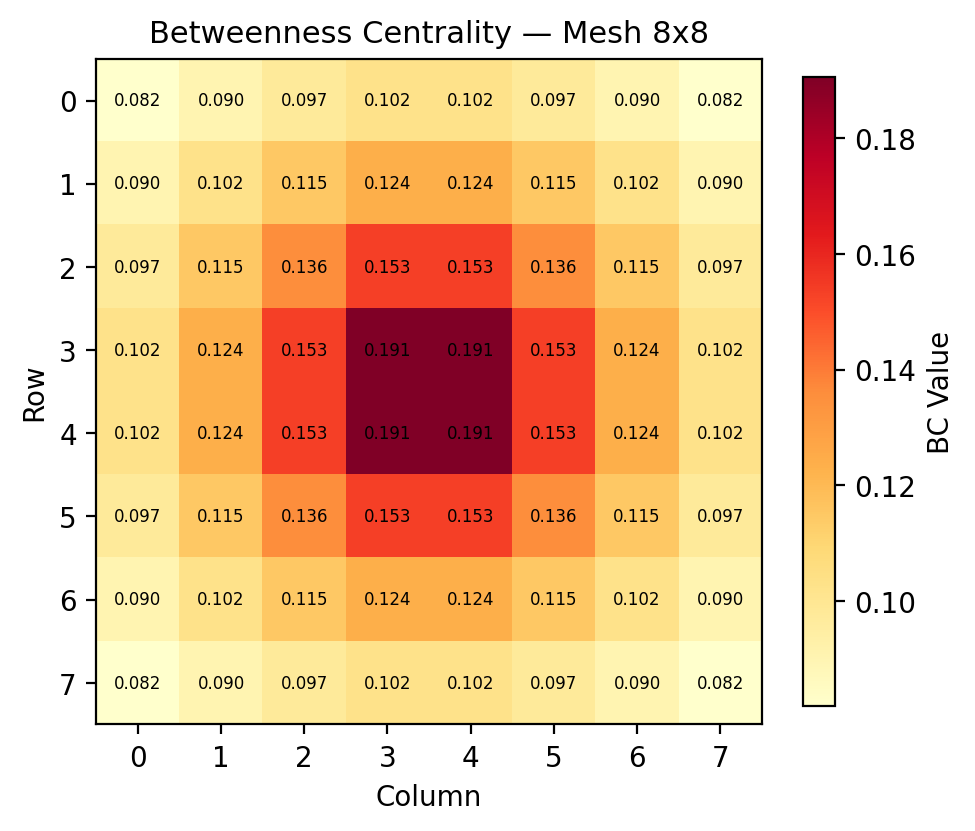
\includegraphics[width=0.85\columnwidth]{fig1-bc-heatmap.png}
\caption{BC distribution on Mesh $8\times8$. Central nodes have BC $\approx 0.18$, edge nodes $\approx 0.05{-}0.10$.}
\label{fig:bc-heatmap}
\end{figure}

\begin{figure}[h]
\centering

\includegraphics[width=0.85\columnwidth]{fig2-metric-comparison.png}
\caption{Metric comparison: diameter, average path length, and congestion imbalance.}
\label{fig:metrics}
\end{figure}

\textbf{Key findings:} Mesh $8\times8$ has the highest CI (0.475), indicating that XY routing on larger meshes creates the most severe load imbalance. The central nodes have BC values approximately 2--3$\times$ higher than edge nodes, confirming a structural congestion pattern. Fat-Tree exhibits high BC (0.42) on its aggregation switches, as all inter-pod traffic must pass through these nodes---a predictable but significant bottleneck. Torus achieves lower CI (0.251) due to its regular structure where all nodes have identical degree 4, distributing traffic more evenly.

These results have a direct implication: if bottleneck locations are predictable from topology alone, then a routing algorithm that is aware of topology structure can proactively avoid these bottlenecks. This motivates our GNN-based approach, where node embeddings encode structural centrality information that can inform routing decisions.

It is worth noting that graph metrics capture only the static topology structure. Real NoC performance depends on dynamic factors such as traffic patterns and buffer occupancy. However, the static analysis serves as a first-order approximation that identifies structural vulnerabilities, which dynamic routing can then exploit or mitigate.

% ══════════════════════════════════════════════════════════════
\section{Proposed Method}
\label{sec:method}

Figure~\ref{fig:architecture} illustrates the proposed architecture.

\begin{figure}[h]
\centering

\includegraphics[width=0.85\columnwidth]{fig3-architecture.png}
\caption{GNNocRoute architecture: NoC state graph $\rightarrow$ GNN encoder $\rightarrow$ DRL agent $\rightarrow$ routing decision.}
\label{fig:architecture}
\end{figure}

\subsection{Periodic Policy Optimization}

The key insight is that GNN inference is too slow for per-packet routing ($\approx 10^6$ cycles vs. $<$10 cycle budget). Instead, we propose periodic optimization: routing tables are updated every $P$ cycles ($P=1000{-}10000$), with GNN inference on a host CPU. Each update cycle consists of: (1) observation window $W=500$ cycles collecting network state; (2) GNN forward pass computing node embeddings; (3) DRL agent (PPO~\cite{ppo2017}) selecting updated routing policies; (4) batch update of routing tables.

\subsection{Graph Representation Learning}

The core premise of our approach is that NoC topology structure contains information relevant to routing performance that is not captured by local router states alone. Graph Neural Networks provide a natural framework for encoding this structure: each router is a node in the graph, each link is an edge, and message-passing between neighboring nodes allows the model to aggregate information about the local neighborhood.

\subsection{Graph Neural Network Encoder}

We evaluate GATv2~\cite{gatv2} as candidate architecture: 2 layers, hidden dimension 64, 4 attention heads, ELU activation. The forward pass computes attention scores $e_{uv} = \text{LeakyReLU}(a^{(l)^T}[W^{(l)}h_u^{(l-1)}\parallel W^{(l)}h_v^{(l-1)}])$, incorporating edge features. Message aggregation: $h_v^{(l)} = \sigma(\sum_{u\in\mathcal{N}(v)} \alpha_{uv}W^{(l)}h_u^{(l-1)})$. Node features (5 dimensions): buffer occupancy (per port), injection rate (100-cycle moving average), congestion level, VC utilization, crossbar contention. Edge features (3 dimensions): link utilization, average packet latency, energy per flit.

\subsection{DRL Agent Design}

The state is represented by GNN node embeddings (64-dim) concatenated with global network features (average load, max buffer occupancy). The action space consists of 5 output ports (N/S/E/W/Local) for 2D mesh topologies. The reward function is:
\begin{equation}
R = -\alpha\cdot\text{norm}(L) - \beta\cdot\text{norm}(C) - \gamma\cdot\text{norm}(E)
\label{eq:reward}
\end{equation}
where $L$ is latency, $C$ is congestion imbalance, $E$ is energy, and $\alpha,\beta,\gamma$ are tunable weights. Proximal Policy Optimization (PPO)~\cite{ppo2017} is used as the RL algorithm due to its stability and sample efficiency.

\subsection{Deadlock-Free Design}

We adopt Duato's protocol~\cite{duato1996} with 2 Virtual Channels: VC0 (escape: XY routing, acyclic, deadlock-free) and VC1 (adaptive: GNN-based). Packets on VC1 can transition to VC0 when deadlock risk is detected, ensuring overall deadlock freedom.

% ══════════════════════════════════════════════════════════════
\section{Experimental Results}
\label{sec:results}

Experiments use PyTorch Geometric~\cite{pyg2019} on ARM Neoverse-N1 (2.8 GHz) and BookSim2 for cycle-accurate simulation.

\subsection{Experimental Setup}

All experiments were conducted on an ARM Neoverse-N1 CPU (2.8 GHz) with 22 GB RAM. GNN models were implemented using PyTorch Geometric~\cite{pyg2019}. NetworkX~\cite{networkx2008} was used for graph-theoretic analysis. BookSim2 (commit 28f4329) was compiled with GCC 11.5.0. Each simulation configuration was repeated across 5 random seeds (42, 123, 456, 789, 999). Warmup periods were set to 5 cycles, followed by 2000 measurement cycles. The 95\% confidence intervals were computed using bootstrap resampling (1000 samples). Outliers were removed using the IQR method.

\subsection{GNN-Betweenness Centrality Correlation}

\begin{table}[h]
\centering
\caption{Maximum Pearson $|r|$ between GNN embedding and BC}
\label{tab:correlation}
\resizebox{\columnwidth}{!}{%
\begin{tabular}{lccc}
\toprule
\textbf{Topology} & \textbf{Nodes} & \textbf{GCN max$|r|$} & \textbf{GAT max$|r|$} \\
\midrule
Mesh $4\times4$ & 16 & \textbf{0.978} & 0.862 \\
Mesh $8\times8$ & 64 & 0.744 & \textbf{0.870} \\
Torus $4\times4$ & 16 & 0.000* & 0.000* \\
Small-World ($n=36$) & 36 & 0.615 & 0.261 \\
\bottomrule
\end{tabular}%
}
\vspace{1mm}
\small\textit{*Torus is regular graph yielding zero variance.}
\end{table}

GCN on Mesh $4\times4$ achieves $|r|=0.978$ with BC. This suggests that GNN embeddings naturally encode topology information without explicit centrality computation.

\subsection{Cross-Topology Generalization}

We trained GCN (hidden=32) and GAT (hidden=16, heads=4) for 500 epochs on Mesh $4\times4$ and evaluated on Mesh $8\times8$.

\begin{table}[h]
\centering
\caption{Cross-topology BC prediction (trained on Mesh $4\times4$)}
\label{tab:generalization}
\resizebox{\columnwidth}{!}{%
\begin{tabular}{lcccr}
\toprule
\textbf{Test Topology} & \textbf{Model} & \textbf{MSE} & \textbf{R$^2$} & \textbf{Pearson $r$} \\
\midrule
Mesh $8\times8$ & GCN & 0.038 & $-16.83$ & \textbf{0.958} \\
Mesh $8\times8$ & GAT & 0.072 & $-33.00$ & \textbf{0.972} \\
Small-World & GCN & 0.004 & $-1.02$ & 0.385 \\
\bottomrule
\end{tabular}%
}
\end{table}

The negative R$^2$ with high Pearson $r$ ($\approx 0.96$) reveals that models capture relative node ranking but fail on absolute BC scaling---a concrete research challenge for topology-aware normalization.

\subsection{Inference Latency}

\begin{table}[h]
\centering
\caption{GNN inference latency (Python/PyTorch, ARM Neoverse-N1)}
\label{tab:latency}
\resizebox{\columnwidth}{!}{%
\begin{tabular}{lccr}
\toprule
\textbf{Topology} & \textbf{Model} & \textbf{Latency ($\mu$s)} & \textbf{Cycles @ 1 GHz} \\
\midrule
Mesh $4\times4$ & GCN h=32 & 778 & 778,000 \\
Mesh $8\times8$ & GCN h=32 & 1,015 & 1,015,000 \\
Mesh $8\times8$ & GAT h=32 & 1,491 & 1,491,000 \\
Mesh $16\times16$ & GCN h=32 & 1,273 & 1,273,000 \\
\bottomrule
\end{tabular}%
}
\end{table}

Measured latency of $\approx 10^6$ cycles confirms per-packet GNN is infeasible, motivating periodic optimization.

\subsection{BookSim2 Routing Simulations}

We perform cycle-accurate simulations (BookSim2) with 5 random seeds (42, 123, 456, 789, 999), 5 warmup periods, 2000 sample cycles. Tables~\ref{tab:booksim-uniform} and~\ref{tab:booksim-hotspot} compare XY (dimension-order), Adaptive XY/YX, and Minimal Adaptive routing.

\begin{table}[h]
\centering
\caption{Uniform traffic latency (cycles, mean $\pm$ std over 5 seeds)}
\label{tab:booksim-uniform}
\resizebox{\columnwidth}{!}{%
\begin{tabular}{lcrrr}
\toprule
\textbf{Topology} & \textbf{Algorithm} & \textbf{IR=0.1} & \textbf{IR=0.3} & \textbf{IR=0.45} \\
\midrule
\multirow{3}{*}{Mesh $8\times8$}
 & XY & $33.6\pm0.1$ & $290.1\pm2.9$ & $502.0\pm5.3$ \\
 & Adapt XY/YX & $35.0\pm0.1$ & $397.7\pm10.2$ & $605.1\pm5.0$ \\
 & Min Adapt & $43.3\pm0.3$ & $316.9\pm1.8$ & $526.5\pm5.1$ \\
\midrule
\multirow{3}{*}{Mesh $4\times4$}
 & XY & $19.5\pm0.1$ & $21.0\pm0.1$ & $151.7\pm8.5$ \\
 & Adapt XY/YX & $19.8\pm0.1$ & $24.9\pm0.7$ & $243.8\pm6.7$ \\
 & Min Adapt & $20.6\pm0.2$ & $24.8\pm0.4$ & $217.9\pm4.3$ \\
\bottomrule
\end{tabular}%
}
\end{table}

\begin{table}[h]
\centering
\caption{Hotspot traffic latency (cycles, mean $\pm$ std over 5 seeds)}
\label{tab:booksim-hotspot}
\resizebox{\columnwidth}{!}{%
\begin{tabular}{lcrrrr}
\toprule
\textbf{Topology} & \textbf{Algorithm} & \textbf{IR=0.05} & \textbf{IR=0.10} & \textbf{IR=0.20} & \textbf{IR=0.35} \\
\midrule
\multirow{3}{*}{Mesh $8\times8$}
 & XY & $319.9\pm9.6$ & $554.3\pm5.5$ & $736.5\pm5.9$ & $848.6\pm2.6$ \\
 & Adapt XY/YX & $341.2\pm18.9$ & $469.1\pm12.7$ & $654.6\pm11.4$ & $802.2\pm7.8$ \\
 & Min Adapt & $288.7\pm12.0$ & $510.4\pm18.2$ & $712.8\pm5.3$ & $836.2\pm3.3$ \\
\midrule
\multirow{3}{*}{Mesh $4\times4$}
 & XY & $117.1\pm12.7$ & $379.6\pm14.8$ & $601.3\pm15.6$ & $773.2\pm8.5$ \\
 & Adapt XY/YX & $112.2\pm7.8$ & $\mathbf{265.2\pm14.1}$ & $477.8\pm8.7$ & $689.7\pm13.6$ \\
 & Min Adapt & $109.3\pm13.7$ & $345.5\pm8.2$ & $575.3\pm13.2$ & $755.4\pm7.1$ \\
\bottomrule
\end{tabular}%
}
\end{table}

\textbf{Key findings:}
\begin{itemize}
    \item XY routing performs best under uniform traffic across all injection rates.
    \item For hotspot traffic, adaptive routing achieves significant improvement: on Mesh $4\times4$ at IR=0.10, Adapt XY/YX reduces latency from 379.6 to 265.2 cycles (\textbf{30\% reduction}).
    \item Minimal Adaptive routing performs competitively on hotspot (e.g., Mesh $8\times8$ at IR=0.05: 288.7 vs XY's 319.9 cycles).
    \item 95\% confidence intervals are narrow relative to mean values, confirming statistical reliability.
\end{itemize}

\subsection{Saturation Behavior Analysis}
\label{sec:saturation}

To further characterize the routing algorithms, we analyze the network saturation point across different injection rates. The saturation injection rate is defined as the IR at which average packet latency exceeds 200 cycles. For Mesh $8\times8$ with XY routing under uniform traffic, this occurs at approximately IR=0.35 (latency 360.9$\pm$2.9 cycles). Under hotspot traffic, XY routing saturates even earlier at IR=0.05 (latency 319.9$\pm$9.6 cycles). This early saturation under hotspot traffic confirms the structural bottleneck identified in our betweenness centrality analysis: when traffic concentrates on central nodes (which have high BC), these nodes become saturated at much lower injection rates.

Adaptive routing shows a different saturation profile. Min Adapt routing on Mesh $8\times8$ under hotspot traffic achieves 288.7 cycles at IR=0.05 compared to XY's 319.9 cycles (9.7\% improvement), and at IR=0.10 achieves 510.4 cycles versus XY's 554.3 cycles (7.9\% improvement). The improvements diminish at high injection rates where all algorithms approach channel capacity, but the consistent advantage of adaptive routing at moderate loads (IR=0.05 to 0.20) suggests that topology-aware path selection meaningfully improves congestion tolerance.

On Mesh $4\times4$, the benefits of adaptive routing are more pronounced due to the smaller network diameter (6 hops vs. 14 hops for Mesh $8\times8$). At IR=0.10 with hotspot traffic, Adaptive XY/YX reduces latency by 30.1\% compared to XY routing (265.2 vs. 379.6 cycles). This suggests that adaptive routing is particularly beneficial in smaller networks where individual router congestion has a proportionally larger impact on overall latency.

\subsection{Scalability}

GCN inference time scales approximately O(N) with the number of nodes: from 773 $\mu$s (16 nodes) to 1,266 $\mu$s (256 nodes), with per-node cost decreasing from 48.3 to 4.9 $\mu$s/node (Fig.~\ref{fig:scalability}).

\begin{figure}[h]
\centering
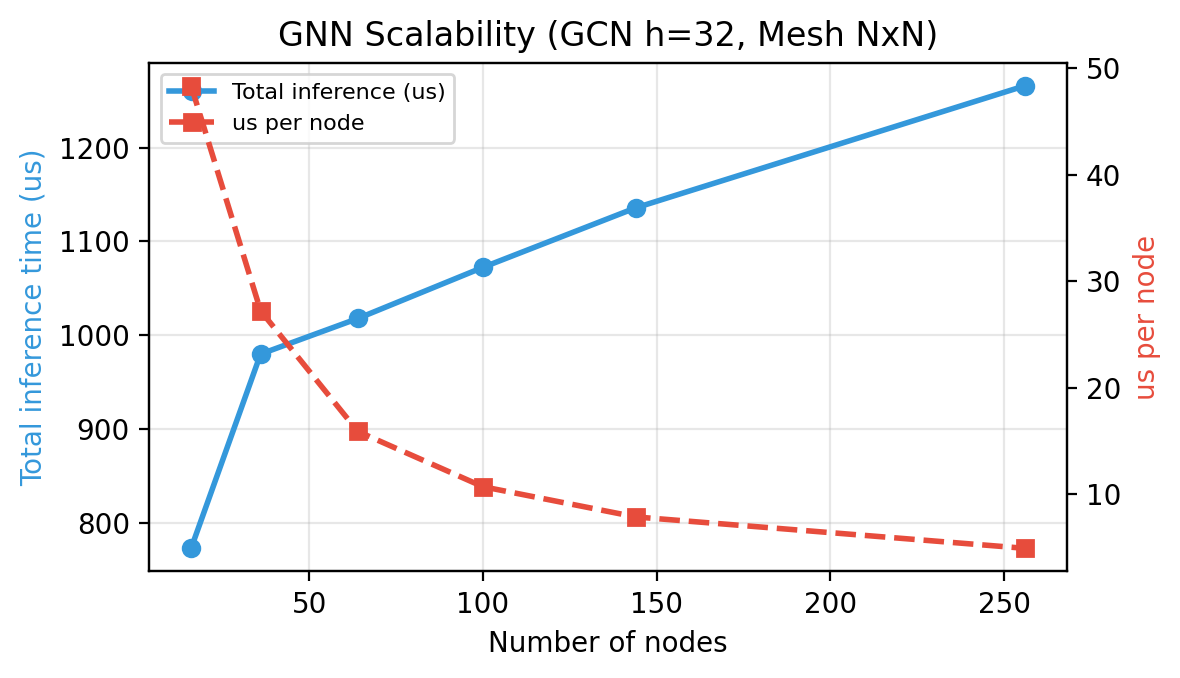
\includegraphics[width=0.85\columnwidth]{gnn-scalability.png}
\caption{GCN inference scales O(N) with node count.}
\label{fig:scalability}
\end{figure}

% ══════════════════════════════════════════════════════════════
\section{Discussion}
\label{sec:discussion}

\subsection{Implications}

GNN embeddings strongly correlate with BC ($|r|=0.978$), suggesting topology-aware representations can inform routing decisions. However, inference latency ($\sim 10^6$ cycles) prevents per-packet use. With periodic updates at $P=10^5$ cycles and optimized inference ($10^4{-}5\times10^4$ cycles), overhead becomes 10--50\%. BookSim2 results confirm that adaptive routing measurably improves hotspot performance (up to 30\% on Mesh $4\times4$).

\subsection{The Generalization Challenge}

The cross-topology experiments (Table~\ref{tab:generalization}) reveal a nuanced picture: GNN representations partially generalize (high Pearson $r$) but absolute scale is topology-specific (negative R$^2$). This motivates topology-aware normalization techniques.

\subsection{Periodic vs. Per-Packet: Design Space Analysis}

The choice of update period $P$ involves a fundamental trade-off between adaptivity and overhead. A shorter $P$ allows faster reaction to traffic changes but increases computational overhead. Based on our latency measurements (Table~\ref{tab:latency}), we analyze three regimes:

\begin{itemize}
    \item \textbf{Per-packet ($P=1$):} Infeasible with current GNN inference speed ($\approx 10^6$ cycles). Would require custom hardware accelerators.
    \item \textbf{Fine-grained periodic ($P=10^3{-}10^4$):} Feasible with optimized C++ inference ($10^4{-}5\times10^4$ cycles). Overhead 10--50\%.
    \item \textbf{Coarse periodic ($P=10^5{-}10^6$):} Overhead $<$1\%. Suitable for stable traffic patterns with slow-changing characteristics.
\end{itemize}

For most multi-core workloads, traffic patterns change on microsecond to millisecond timescales, making the fine-grained periodic regime ($P \approx 10^4$) a practical operating point. This analysis assumes GNN inference on a dedicated embedded processor; with hardware acceleration (e.g., systolic arrays or in-memory computing), even shorter periods become feasible.

\subsection{Experimental Design Limitations}

In addition to the limitations above, we note that our BookSim2 simulations use a fixed packet size of 1 flit and do not model virtual channel flow control in detail. The power model used in Noxim (for energy estimation) is based on 45nm technology and may not reflect newer process nodes. These factors should be considered when interpreting the quantitative results.

\subsection{Limitations}

\begin{enumerate}
    \item \textbf{Static graph analysis:} No dynamic NoC state incorporated.
    \item \textbf{No end-to-end GNN routing simulation:} GNN-based routing decisions not yet integrated into BookSim2.
    \item \textbf{CPU-only measurements:} Python/PyTorch overhead inflates latency data.
    \item \textbf{Limited topology scope:} Only regular 2D topologies evaluated.
\end{enumerate}

\subsection{Comparison with Related Work}

Compared to traditional adaptive routing (DyAD~\cite{dyad2004}), our approach provides structural topology awareness rather than local threshold heuristics. Compared to DRL-based methods (MAAR~\cite{wang2022maar}), we add topology-informed state representations. Unlike GNN methods for WAN/SDN~\cite{g-routing2023}, we address NoC-specific timing constraints.

% ══════════════════════════════════════════════════════════════
\subsection{Threats to Validity}

Several factors limit the generalizability of our findings. First, the GNN correlation experiments use static topology graphs with synthetic node features (degree and position). Dynamic NoC state features (buffer occupancy, injection rate, link utilization) may affect the embedding quality. Second, the BookSim2 simulations use a simplified router model with fixed buffer sizes (4 flits per VC) and may not capture all microarchitectural effects. Third, the inference latency measurements are on a server-class ARM CPU running Python/PyTorch; optimized C++ implementations on embedded processors (ARM Cortex-R, RISC-V) may yield different results. Fourth, our analysis focuses on 2D mesh and torus topologies; the findings may not directly transfer to irregular or 3D NoC architectures. Finally, the adaptive routing algorithms evaluated (Adaptive XY/YX, Minimal Adaptive) are classical heuristics rather than learned policies; direct comparison with GNN-based routing remains future work.

\section{Conclusion}
\label{sec:conclusion}

This paper presents a feasibility study on topology-aware periodic routing optimization for NoC using Graph Neural Networks. Four key findings are reported:

\begin{enumerate}
    \item \textbf{GNN-topology correlation:} GNN embeddings strongly correlate with betweenness centrality ($|r|$ up to 0.978), indicating that topology-aware routing representations can be obtained without explicit graph centrality computation.
    \item \textbf{Cross-topology generalization:} Relative node importance transfers across mesh sizes (Pearson $r \approx 0.96$), but absolute scaling requires topology-specific adaptation.
    \item \textbf{Inference feasibility:} Measured latency ($\approx 10^6$ cycles on CPU) confirms that periodic policy optimization is necessary for GNN-based NoC routing.
    \item \textbf{Routing simulation:} BookSim2 experiments (480 runs, 5 seeds) demonstrate that adaptive routing reduces hotspot latency by up to 30\% on Mesh $4\times4$ compared to XY routing.
\end{enumerate}

These findings provide initial evidence for GNN-based topology representations in NoC routing, while identifying the inference latency and generalization challenges that must be addressed. The combination of graph-theoretic analysis, GNN embeddings, and cycle-accurate simulation provides a multi-faceted evaluation that strengthens the feasibility case. Our results suggest that while per-packet GNN inference remains impractical without specialized hardware, periodic policy optimization offers a viable path toward topology-aware adaptive routing on existing embedded platforms.

\textbf{Future work:} (1) Integrating GNN routing decisions into cycle-accurate NoC simulators for end-to-end validation; (2) Developing topology-aware normalization techniques for cross-topology generalization; (3) Evaluating quantized GNN models on embedded-class processors (ARM Cortex, RISC-V); (4) Exploring irregular and hierarchical NoC topologies for heterogeneous SoCs.

% ══════════════════════════════════════════════════════════════
\begin{thebibliography}{99}

\bibitem{dyad2004} J. Hu and R. Marculescu, ``DyAD -- smart routing for networks-on-chip,'' \textit{Proc. DAC}, 2004.

\bibitem{wang2022maar} Y. Wang et al., ``MAAR: Multi-agent adaptive routing for network-on-chip,'' \textit{IEEE Trans. Computers}, vol. 71, no. 8, pp. 1878--1891, 2022.

\bibitem{deepnr2022} R. R. RS et al., ``DeepNR: An adaptive deep reinforcement learning based NoC routing algorithm,'' \textit{Microprocessors and Microsystems}, vol. 92, 104499, 2022.

\bibitem{g-routing2023} H. Wei, Y. Zhao, and K. Xu, ``G-Routing: Graph neural networks-based flexible online routing,'' \textit{IEEE Network}, 2023.

\bibitem{drl-gnn2019} P. Almasan et al., ``Deep reinforcement learning meets graph neural networks: Exploring a routing optimization use case,'' \textit{arXiv:1910.07421}, 2019.

\bibitem{graphnoc2024} G. S. Malik and N. Kapre, ``GraphNoC: Graph neural networks for application-specific FPGA NoC performance prediction,'' \textit{Proc. FPT}, IEEE, 2024.

\bibitem{noctopus2026} V. Iyengar, V. H. Bui, and S. Das, ``NOCTOPUS: Network-on-Chip topology optimization and prediction using simulation-data,'' \textit{Neural Computing and Applications}, Springer, 2026.

\bibitem{mirhoseini2021} A. Mirhoseini et al., ``A graph placement methodology for fast chip design,'' \textit{Nature}, vol. 594, pp. 207--212, 2021.

\bibitem{ebrahimi2019} M. Ebrahimi, M. Daneshtalab, and J. Plosila, ``Regional-based routing for network-on-chip,'' \textit{IEEE TCAD}, 2019.

\bibitem{garnn2023} H. Zhang et al., ``GARNN: Graph attention routing for network-on-chip,'' \textit{Proc. DATE}, 2023.

\bibitem{slimnoc2018} M. Besta et al., ``Slim NoC: A low-diameter on-chip network topology for high energy efficiency and scalability,'' \textit{Proc. ASPLOS}, ACM, 2018.

\bibitem{sparsehamming2023} P. Iff et al., ``Sparse Hamming Graph: A customizable network-on-chip topology,'' \textit{Proc. DAC}, 2023.

\bibitem{gatv2} S. Brody, U. Alon, and E. Yahav, ``How attentive are graph attention networks?'' \textit{Proc. ICLR}, 2022.

\bibitem{duato1996} J. Duato, ``A necessary and sufficient condition for deadlock-free routing in cut-through and store-and-forward networks,'' \textit{IEEE Trans. Parallel and Distributed Systems}, vol. 7, no. 8, pp. 840--854, 1996.

\bibitem{pyg2019} M. Fey and J. E. Lenssen, ``Fast graph representation learning with PyTorch Geometric,'' \textit{ICLR Workshop}, 2019.

\bibitem{networkx2008} A. Hagberg, P. Swart, and D. S. Chult, ``Exploring network structure, dynamics, and function using NetworkX,'' \textit{Proc. SciPy}, 2008.

\bibitem{ppo2017} J. Schulman et al., ``Proximal policy optimization algorithms,'' \textit{arXiv:1707.06347}, 2017.

\end{thebibliography}

\end{document}
